%%%%%%%%%%%%%%%%%%%%%%%%%%%%%%%%%%%%%%%%%%%%%%%%%%%%%
%%% Task 2 %%%%%%%%%%%%%%%%%%%%%%%%%%%%%%%%%%%%%%%%%%
%%%%%%%%%%%%%%%%%%%%%%%%%%%%%%%%%%%%%%%%%%%%%%%%%%%%%
\task{Series DC machine}

%%%%%%%%%%%%%%%%%%%%%%%%%%%%%%%%%%%%%%%%%%%%%%
\taskGerman{Reihenschluss-Gleichstrommaschine}
%%%%%%%%%%%%%%%%%%%%%%%%%%%%%%%%%%%%%%%%%%%%%%

Electric vehicle drives were used in mines at an early historic stage in order to avoid exhausts  from combustion engines in the tunnels. Historically, series DC machines were used for this purpose, such as the machine with the parameters summarized in the following table.

\begin{germanblock}
    In Bergwerken sind bereits früh elektrische Fahrzeugantriebe eingesetzt worden, um Abgase von Verbrennungsmotoren in den Stollen zu vermeiden. Historisch wurden hierfür u.~a. Reihenschluss-Gleichstrommaschinen verwendet, wie beispielsweise die Maschine mit den Parametern aus der nachfolgenden Tabelle.
\end{germanblock}
\begin{table}[htb]
    \caption{DC machine parameters.}
    \centering
    \begin{tabular}{lll}\toprule
    Symbol  & Description       & Values \\
    \midrule
    $U_{\mathrm{n}}$    & Nominal voltage           & $\SI{440}{\volt}$ \\
    $I_{\mathrm{n}}$    & Nominal armature current           & $\SI{500}{\ampere}$ \\
    $T_{\mathrm{n}}$    & Nominal torque             & $\SI{1407}{\newton\meter}$ \\
    $R_\mathrm{a}$ & Armature resistance & \SI{0.02}{\ohm}\\
    $R_\mathrm{f}$ & Field resistance & \SI{0.025}{\ohm}\\
    $L_\mathrm{a}$ & Armature inductance & \SI{2}{\milli\henry}\\
    $L_\mathrm{f}$ & Field inductance & \SI{8}{\milli\henry}\\
    \bottomrule
    \end{tabular}
    \label{tab:characteristicsIM_task3}
\end{table}


\subtask{Draw the equivalent circuit diagram of the series DC machine.}{1}

\subtaskGerman{Zeichnen Sie das Ersatzschaltbild der Reihenschluss-Gleichstrommaschine.}

\begin{solutionblock}
\begin{solutionfigure}[ht]
    \centering
    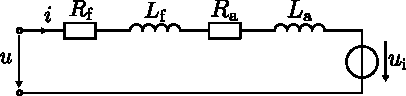
\includegraphics[width=0.6\linewidth]{fig/ECD_DC_series.pdf}
    \caption{Equivalent circuit diagram of the series DC machine}
    \label{fig:ECD_DC_series}
\end{solutionfigure}
\end{solutionblock}

\subtask{Determine the effective field inductance $L'_\mathrm{f}$ and the effective flux linkage $\psi'_\mathrm{f}$ for the nominal steady-state operating point.}{2}%
\begin{hintblock}
if and if only you are not able to solve this task, use $L'_\mathrm{f} = \SI{8}{\milli\henry}$ and $\psi'_\mathrm{f} = \SI{4}{\volt\second}$ as a substitute result for the subsequent tasks.
\end{hintblock}

\subtaskGerman{Bestimmen Sie die effektive Erregerinduktivität $L'_\mathrm{f}$ und die effektive Flussverkettung $\psi'_\mathrm{f}$ für den nominellen Arbeitspunkt im stationären Zustand.}%
\begin{germanhintblock}
nur für den Fall, dass Sie kein Ergebnis ermitteln können, verwenden Sie $L'_\mathrm{f} = \SI{8}{\milli\henry}$ und $\psi'_\mathrm{f} =$ \SI{4}{\volt\second} für die nachfolgenden Aufgaben.
\end{germanhintblock}


\begin{solutionblock}
    The series DC machine torque equation reads
    $$
    T = L'_\mathrm{f} I^2
    $$
    allowing to calculate the effective field inductance utilizing the nominal values of the machine:
    $$
    L'_\mathrm{f} = \frac{T_\mathrm{n}}{I^2_\mathrm{n}} = \SI{5.63}{\milli\henry}.
    $$
    The effective flux linkage then results in
    $$
    \psi'_\mathrm{f,n} = L'_\mathrm{f}I_\mathrm{n}=\SI{2.81}{\volt\second}.
    $$
\end{solutionblock}

\subtask{What is the machine's nominal speed $n_\mathrm{n}$ and efficiency $\eta_\mathrm{n}$?}{2}
\subtaskGerman{Wie hoch ist die Nenndrehzahl $n_\mathrm{n}$ und der nominelle Wirkungsgrad $\eta_\mathrm{n}$ der Maschine?}


\begin{solutionblock}
    First, the induced voltage is calculated via
    $$
    U_\mathrm{i,n} = U_\mathrm{n} - (R_\mathrm{a} + R_\mathrm{f})I_\mathrm{n} = \SI{417.5}{\volt}.
    $$
    The nominal angular velocity is
    $$
    \omega_\mathrm{n} = \frac{U_\mathrm{i,n}}{\psi'_\mathrm{f,n}} = \SI{148.6}{\per\second}
    $$
    resulting in
    $$
    n_\mathrm{n} = \omega_\mathrm{n} \frac{60}{2\pi}\frac{\si{\second}}{\si{\minute}} = \SI{1418.8}{\per\minute}. 
    $$
    For determining the nominal efficiency, we first calculate the nominal electrical and mechanical powers
    $$
    P_\mathrm{el,n} = U_\mathrm{n}I_\mathrm{n} = \SI{220}{\kilo\watt}, \quad P_\mathrm{me,n} = T_\mathrm{n}\omega_\mathrm{n} = \SI{209.1}{\kilo\watt}
    $$
    leading to
    $$
    \eta_\mathrm{n} = \frac{P_\mathrm{me,n}}{P_\mathrm{el,n}} = \SI{95.05}{\percent}.
    $$
\end{solutionblock}

\subtask{Due to a fault in the cooling system, the dissipated power losses must be reduced to $\nicefrac{1}{4}$ of the nominal rating to prevent overheating. What are the achievable torque and mechanical power in this scenario assuming that the ohmic losses dominate the machine's loss characteristic? What mechanical issue could occur in this new operating point?}{3}
\subtaskGerman{Aufgrund eines Fehlers im Kühlsystem muss die Verlustleistung auf $\nicefrac{1}{4}$ des Nennbetriebs reduziert werden, um eine Überhitzung zu vermeiden. Wie hoch sind das erreichbare Drehmoment und die mechanische Leistung in diesem Szenario, wenn man davon ausgeht, dass die ohmschen Verluste dominierend sind? Welches mechanische Problem könnte in diesem neuen Arbeitspunkt auftreten?}

\begin{solutionblock}
As the power losses
$$
P_\mathrm{l} = (R_\mathrm{a}+R_\mathrm{f})I^2
$$
must be quartered, the machine's input current must be halved. Hence, the achievable torque results in
$$
T = L'_\mathrm{f}\left(\frac{I_\mathrm{n}}{2}\right)^2=\frac{1}{4}T_\mathrm{n} = \SI{351.8}{\newton\meter}. 
$$
Due the the halved input current, the induced voltage as well as the effective flux linkage are varying:
$$
U_\mathrm{i} = U_\mathrm{n} - (R_\mathrm{a}+R_\mathrm{f})\left(\frac{I_\mathrm{n}}{2}\right) = \SI{428.8}{\volt}, \quad \psi_\mathrm{f}' = L'_\mathrm{f} \left(\frac{I_\mathrm{n}}{2}\right) = \SI{1.41}{\volt\second}.
$$
The resulting speed is
$$
n = \frac{U_\mathrm{i}}{\psi_\mathrm{f}'} \frac{60}{2\pi}\frac{\si{\second}}{\si{\minute}} = \SI{2904.1}{\per\minute}
$$
leading to the mechanical power of 
$$
P_\mathrm{me} = \omega T = \SI{106.99}{\kilo\watt}.
$$
Since the rotational speed of the machine has more than doubled compared to its nominal value, mechanical integrity problems could occur due to the much higher centrifugal forces occurring within the rotor. Also, the bearings must withstand the higher rotational speed. 
\end{solutionblock}

\subtask{What steady-state starting current can be expected when the nominal machine voltage is applied from the stall position? After what time interval $\Delta T$ is $\SI{95}{\percent}$ of this steady-state value reached when starting from an entirely currentless, non-rotating machine?}{2}
\subtaskGerman{Mit welchem stationären Anlaufstrom ist zu rechnen, wenn die nominelle Maschinenspannung ab Stillstand angelegt wird? Nach welchem Zeitintervall $\Delta T$ ist $\SI{95}{\percent}$ dieses stationären Endwerts erreicht, wenn der Anlauf von einer völlig stromlosen und stillstehenden Maschine startet?} 

\begin{solutionblock}
    During start up, the mechanical speed is zero and the entire machine's voltage drops via the armature and field resistance leading to
    $$
    I_0 = \frac{U_\mathrm{n}}{R_\mathrm{a}+R_\mathrm{f}} =\SI{9.78}{\kilo\ampere}.
    $$
    The DC series machine's ECD represents an ohmic-inductive element with
    $$
    R = R_\mathrm{a}+R_\mathrm{f}, \quad L = L_\mathrm{a}+L_\mathrm{f}.
    $$
    The resulting time constant of this circuit is
    $$
    \tau = \frac{L}{R} = \SI{0.22}{\second}.
    $$
    Based on the exponentially limited increase in the machine current, \SI{95}{\percent} of the final value is reached after $3\tau$, i.e.,
    $$
    \Delta T = 3\tau = \SI{0.66}{\second}.
    $$
\end{solutionblock}

\subtask{What dropping resistor must be added to the machine's circuit to limit the starting current to twice the nominal value?}{1}
\subtaskGerman{Welcher Vorwiderstand ist einzubringen, um den Anlaufstrom auf das Doppelte des Nennwerts zu begrenzen?}
\begin{solutionblock}
    Considering an additional dropping resistor to limit the starting current to twice the nominal current results in
    $$
    2I_\mathrm{n} = \frac{U_\mathrm{n}}{R_\mathrm{a}+R_\mathrm{f}+R_\mathrm{d}}
    $$
    and delivering
    $$
    R_\mathrm{d} = \frac{U_\mathrm{n}}{2 I_\mathrm{n}} - R_\mathrm{a} -R_\mathrm{f} = \SI{0.395}{\ohm}. 
    $$
\end{solutionblock}